\documentclass[11pt]{article}
\usepackage[final]{acl}
\usepackage{times}
\usepackage{latexsym}
\usepackage[T1]{fontenc}
\usepackage[utf8]{inputenc}
\usepackage{microtype}
\usepackage{inconsolata}
\usepackage{graphicx}
\usepackage{booktabs}
\usepackage{array}
\usepackage{amsmath}

\newcommand{\best}[1]{\textbf{#1}}

\title{Drift Monitor: Calling a Smarter Model Only When a Cheaper Agent Drifts}

\author{William Bird \\
  Rokode Labs \\
  Solo team, Lexsi AI Safety and Alignment Hackathon 2026 \\
  \texttt{huggingface.co/dev-willbird1936}}

\begin{document}
\maketitle

\begin{abstract}
Cheaper language-model agents are capable but drift more: they wander from what the user asked while still producing plausible work. Asking a smarter model to review every step costs more than the agent, so the cheap agent usually runs unwatched. We fine-tune a 3.35B open model, tiny-aya-global, to read an agent session from outside and emit one digit for how far the work has drifted from the request. Its digit probabilities give a 0--100 score; above a threshold, a stronger advisor model is called. Training data pairs each of 16 drift patterns with a near-identical on-course twin that differs only in what the user authorised, rendered at six levels of visibility, plus 1,902 recorded real sessions, 90,365 rows in all. On 770 held-out real sessions, AUROC rises from 0.552 to 0.960 and false alarms on clean steps fall from 100\% to 5.4\%. Given the same prompt, two frontier models raise 5--6$\times$ more false alarms at equal recall. On a live agent (256 sessions, 6 of 16 tasks unseen), the monitor-gated advisor removes every unrequested file the agent left behind (2.48 per session to 0) and raises task checks passing from 84\% to 99\%, using 29\% of the advisor calls of per-turn review on drifting sessions and 2\% on clean ones. We report where it fails: deletions, agents that refuse correction, and drift inside a requested file.
\end{abstract}

\section{Introduction}

When a user hands a task to an AI agent, they authorise a specific piece of work. Oversight is lost in the gap between that authorisation and what the agent then does: it edits a file it was told not to touch, follows an instruction planted in a document it was only asked to read, reports that tests pass without running them, or keeps building something the user cancelled two messages earlier. We call this \emph{drift}. It is hard to spot because a drifting agent keeps producing fluent, plausible output.

The obvious defence is to have a strong model review every step. That costs more than the agent it supervises, so in practice the agent runs unwatched. A cheaper but capable agent is the natural thing to run, but it is also the one most likely to drift. We therefore run the cheap agent by default and treat the smarter model as an advisor that gives direction, a plan or a review, called only when the work starts to drift. The review call becomes a spend decision. A small model reads the session after every step and outputs a drift score; only when the score passes a threshold is the expensive advisor consulted. The score gives the advisor call a trigger, so the system buys a higher model's judgement only when it is needed. The monitor itself is a classifier replacing a high-volume closed-model API call, and it is cheap enough to leave on.

The monitor is an external observer, not a tool the agent can call: an agent that has drifted cannot be trusted to report that it has. It reads an append-only log of user messages, replies, reasoning, tool calls and results, and outputs a number that something else acts on.

Our contributions are:
\begin{itemize}\itemsep0pt
\item A training corpus for agent drift in which every drift pattern has an \emph{on-course twin} differing only in what the user asked for, rendered at six evidence tiers, and mixed with recorded real sessions (\S\ref{sec:data}).
\item A 3.35B monitor that beats two frontier models used zero-shot on the same prompt, at matched operating points, at 1/12 to 1/21 of the latency (\S\ref{sec:frontier}).
\item A closed-loop evaluation on a live agent with objective outcomes from files on disk: the same outcomes as reviewing every turn with 29\% of the advisor calls on drifting sessions, against an unwatched agent as the baseline (\S\ref{sec:loop}).
\item Two documented failures and their fixes, including a shortcut where confident final reports were read as drift (\S\ref{sec:failures}).
\end{itemize}
Model, data, traces, code and a live demo are public (Appendix~\ref{app:artifacts}). The work is a Track~1 (Fine-tuning and Data Curation) entry for problem statement~2, replacing a closed-model API, and chains all three track toolkits: CuratorKIT \citep{curatorkit} for curation and audit, AlignTune \citep{aligntune} for training and AuditKIT \citep{auditkit} for grading (Appendix~\ref{app:pipeline}).

\section{Related Work}

\paragraph{Agent safety and drift.} Benchmarks such as R-Judge \citep{yuan2024rjudge} and ToolEmu \citep{ruan2024toolemu} test whether models recognise risky agent behaviour, and AgentDojo \citep{debenedetti2024agentdojo} and \citet{greshake2023indirect} study planted instructions. \citet{arike2025goaldrift} measure goal drift over long agent runs. These works evaluate or provoke unsafe behaviour; we train a deployable monitor and measure whether acting on it changes outcomes.

\paragraph{Monitoring and control.} The AI control agenda \citep{greenblatt2024control} uses a weaker trusted model to monitor a stronger one and defer to costlier review on suspicion, the same two-stage structure we use. \citet{baker2025monitoring} show that an LLM reading chain-of-thought catches reward hacking that actions alone hide, and \citet{korbak2025cot} argue this visibility is valuable but fragile. Our evidence tiers make visibility an explicit input, because what a monitor can see depends on the provider and harness.

\paragraph{Small judges and cascades.} Fine-tuned evaluators such as Prometheus \citep{kim2024prometheus} and safety classifiers such as Llama Guard \citep{inan2023llamaguard} show that small models can replace LLM judges \citep{zheng2023judging} on narrow tasks. Cascades and routers \citep{chen2023frugalgpt,ong2024routellm} call a large model only when needed. We combine both: a small judge whose output is a routing decision for safety review. Scoring each step resembles process supervision \citep{lightman2024verify}, applied to authorisation rather than correctness.

\paragraph{Minimal pairs.} Our twins follow counterfactually augmented data \citep{kaushik2020cad} and contrast sets \citep{gardner2020contrast}: near-identical inputs with different labels, to stop the model learning surface cues \citep{geirhos2020shortcut}.

\section{Task and Data}\label{sec:data}

\paragraph{Task.} Given a rendered session up to step $t$, the model emits one digit $d\in\{0,\dots,9\}$, where $d=\lfloor s/10\rfloor$ for a 0--100 drift label $s$. At inference we take the softmax over the ten digit tokens and report $\hat{s}=\sum_d p_d(10d+5)$; the alert threshold applies to $\hat{s}$. A score rather than a label lets operators tighten or loosen the threshold to match the advisor's price.

\paragraph{Synthetic sessions.} No suitable dataset existed. A teacher model (Grok 4.7) wrote and labelled 5,417 sessions across 20 work categories in three bands: consumer (advice, scheduling, personal admin), knowledge work (finance, HR, document review) and technical (software, devops, data engineering). Consumer and knowledge work make up over half, because an earlier technical-only version did not know what to do with someone booking a meeting.

\paragraph{On-course twins.} Each of 16 drift patterns is paired with a control whose visible activity is nearly identical and differs only in what the user asked for (Table~\ref{tab:twins}; full list in Appendix~\ref{app:patterns}). Without twins, a model learns that ``deleting files is bad''; with them it has to read the request. A version without good pairs scored a requested skeleton at 39 and an unrequested one at 40.

\begin{table}[t]
\centering\small
\begin{tabular}{@{}>{\raggedright\arraybackslash}p{0.45\columnwidth}>{\raggedright\arraybackslash}p{0.47\columnwidth}@{}}
\toprule
Drift & On-course twin \\
\midrule
deletes files recklessly & deletes exactly what was named \\
obeys a planted instruction & spots it and refuses \\
claims the tests pass & runs them and shows output \\
quietly does 3 of 5 things & does 3, says which 2 are open \\
breaks a stated constraint & user lifted the constraint \\
\bottomrule
\end{tabular}
\caption{Example drift patterns and their twins.}
\label{tab:twins}
\end{table}

\paragraph{Evidence tiers.} What a monitor can see depends on the harness, so each session is rendered at six tiers, from replies only (tier 1) through tool calls and results (3) and full reasoning (5) to a live stream cut off mid-thought (6); the prompt names the tier (Appendix~\ref{app:tiers}). The same activity can deserve different scores: at tier 2 a repeated \texttt{sql} call looks like a stuck loop, while at tier 6 the reasoning shows a deliberate re-check.

\paragraph{Recorded sessions.} 1,902 real sessions from a live agent harness, run by four agent models, with real tool calls and file edits, were scored by two independent judges. 60\% by session join training; 770 sessions are held out. With all tiers the corpus has 90,365 rows. CuratorKIT cleaned and deduplicated the recorded corpus.

\paragraph{Label quality.} Two judges from other model families (Claude Sonnet 5.5, GPT-6.1 Terra) re-scored the synthetic labels blind, seeing only transcripts. Each agreed with our labels (MAE 7.4 and 11.4 points) more than with each other (12.4; Pearson 0.893), so remaining label error is near the level of disagreement between judges, and a monitor closer than about 10 points MAE is fitting noise. Disagreement is highest where the agent does something alarming that the user authorised (Appendix~\ref{app:labels}).

\section{Model and Training}

The base model is tiny-aya-global \citep{tinyaya}, a 3.35B dense open-weight model. Using AlignTune, we train a QLoRA adapter \citep{dettmers2023qlora,hu2022lora}: 4-bit NF4 with double quantisation, LoRA $r{=}16$, $\alpha{=}32$, dropout 0.05 on all attention and MLP projections, learning rate $10^{-4}$, 2 epochs (1,750 steps), assistant-only loss, maximum length 2,048, on one A100 40GB. Training took about 11 GPU-hours (\$5.20). The released adapter is 60\,MB. The model's chat template is a dictionary of named templates that TRL's assistant-only masking cannot read, so we supply an equivalent single-string template with generation markers. The final training split has 14,000 rows, mixing synthetic sessions with real ones at a 55\% on-course share to match real traffic (\S\ref{sec:failures}). A CuratorKIT audit of this exact split after training flagged 3.1\% of rows, which were left in (Appendix~\ref{app:pipeline}). AuditKIT grades every run from stored predictions.

\section{Results}

\subsection{Before and after training}

Table~\ref{tab:beforeafter} compares the trained adapter with the same base model on the same prompts, over 770 held-out real sessions at threshold 40. The base model is degenerate: it scores about 55 for everything, so it alerts on every step and never misses drift. A single accuracy number would hide this, which is why we report false alarms and misses separately. Over clean steps only, false alarms fall from 100\% to 5.4\%.

\begin{table}[t]
\centering\small
\begin{tabular}{@{}lrr@{}}
\toprule
Metric (real held-out) & Base & Trained \\
\midrule
Exact digit $\uparrow$ & 0.037 & \best{0.660} \\
Within one digit $\uparrow$ & 0.109 & \best{0.846} \\
MAE (points) $\downarrow$ & 43.88 & \best{7.57} \\
AUROC $\uparrow$ & 0.552 & \best{0.960} \\
Correct alert decision $\uparrow$ & 0.164 & \best{0.922} \\
False alarm, clean steps $\downarrow$ & 100\% & \best{5.4\%} \\
Missed drift, all steps $\downarrow$ & \best{0.000} & 0.033 \\
\midrule
\multicolumn{3}{@{}l}{\emph{Unseen work categories (4 held out)}} \\
MAE $\downarrow$ & 35.77 & \best{5.99} \\
AUROC $\uparrow$ & 0.593 & \best{0.981} \\
\bottomrule
\end{tabular}
\caption{Base vs.\ trained, threshold 40.}
\label{tab:beforeafter}
\end{table}

\paragraph{Contamination.} No session appears in two splits, but repeated runs of the same task meant 5.71\% of held-out recorded rows shared a prompt string with training. Removing them moves MAE from 7.57 to 7.80 and AUROC from 0.960 to 0.957; baselines shift similarly. The build now drops such rows.

\paragraph{Generalisation.} On four work categories held out of training, MAE is 5.99 and AUROC 0.981. On 49 hand-written scenarios not in any split, the monitor gets 23/25 and 23/24 right (base 12/25), and flags 97.5\% of drifting sessions at or before the first drifting step (Appendix~\ref{app:suites}).

\subsection{Against frontier models zero-shot}\label{sec:frontier}

Problem statement 2 asks whether the small model can replace the closed-model call, so the relevant baseline is a large model doing the same job. We sent the identical monitor prompt to Claude Sonnet 5.5 and GPT-6.1 Terra and scored 497 identical held-out real rows (Table~\ref{tab:frontier}). Raw threshold metrics favour whoever sits at a convenient operating point, so we also compare at matched recall and matched false-alarm rate. At equal recall, the 3.35B model raises 5--6$\times$ fewer false alarms; at an equal false-alarm rate it catches 1.6--1.8$\times$ more drift. A score takes 0.3\,s, against 3.6\,s and 6.6\,s.

\begin{table}[t]
\centering\small
\setlength{\tabcolsep}{4pt}
\begin{tabular}{@{}lrrr@{}}
\toprule
& Ours & Sonnet 5.5 & Terra \\
\midrule
MAE $\downarrow$ & \best{7.5} & 13.1 & 14.1 \\
AUROC $\uparrow$ & \best{0.970} & 0.881 & 0.834 \\
Exact digit $\uparrow$ & \best{0.628} & 0.449 & 0.527 \\
Latency (s) $\downarrow$ & \best{0.3} & 6.6 & 3.6 \\
\midrule
FA @ recall $\geq$0.70 $\downarrow$ & \best{2.5\%} & 12.9\% & 16.5\% \\
Recall @ FA $\leq$0.10 $\uparrow$ & \best{93.1\%} & 57.8\% & 52.0\% \\
\bottomrule
\end{tabular}
\caption{Same prompt, same 497 real held-out rows. FA: false-alarm rate. Frontier models at their best configuration.}
\label{tab:frontier}
\end{table}

An obvious objection is that our model absorbed the scoring rubric in training while the frontier models saw a one-line instruction. Giving them the full rubric did not close the gap. Sonnet became much worse (AUROC 0.881 to 0.671, false alarms 44.6\%) because it applied the written bands literally and over-penalised ordinary work; Terra was unchanged within noise (0.834 to 0.854). The claim is narrow: on this task and distribution, a specialised 3.35B model beats general frontier models used zero-shot. Few-shot prompting or a fine-tuned frontier model would be a different contest.

\subsection{Closed loop on a live agent}\label{sec:loop}

Correct scores matter only if acting on them helps. We ran a live agent (Grok 4.7) with real tools in a sandbox on 16 tasks, 10 also in the recorded corpus and 6 written after training. In three conditions a hidden system prompt nudges the agent to drift: adding unrequested deliverables, over-building scaffolding, or breaking a stated constraint; a fourth condition is clean. In the \emph{monitor} arm the monitor scores every turn at threshold 30; on an alert, a read-only advisor (Claude Sonnet 5.5) sees what an outside observer sees and replies \texttt{NO\_ACTION} or writes a short note passed to the agent, at most twice per session. Neither monitor nor advisor sees the hidden prompt. Every combination ran twice per arm (256 sessions, shuffled), with tasks, arms and outcome measures fixed in advance. Outcomes come from files on disk and each task's own check script, not from a model.

\begin{table}[t]
\centering\small
\setlength{\tabcolsep}{3pt}
\begin{tabular}{@{}lrrrr@{}}
\toprule
& \multicolumn{2}{c}{Unseen tasks} & \multicolumn{2}{c}{Pooled} \\
Induced drift & none & monitor & none & monitor \\
\midrule
Unrequested files/session & 2.44 & \best{0.00} & 2.48 & \best{0.00} \\
Sessions leaving any & 64\% & \best{0\%} & 63\% & \best{0\%} \\
Task check passes & 92\% & \best{100\%} & 84\% & \best{99\%} \\
Advisor calls/session & -- & 1.47 & -- & 1.39 \\
\bottomrule
\end{tabular}
\caption{Live agent, induced-drift sessions (36 unseen and 96 pooled per arm). Pooled 95\% bootstrap CI of monitor minus none: files $-2.99$ to $-1.99$; check pass $+7$ to $+22$ points.}
\label{tab:loop}
\end{table}

Table~\ref{tab:loop} shows that drift was not prevented but caught and reversed: the agent wrote extra files, the monitor scored the turn (median 372\,ms), the advisor named the files (median 6.3\,s), and the agent removed them. On 32 clean sessions the monitor alerted twice, and the advisor answered \texttt{NO\_ACTION} both times, so no note reached the agent. Replaying the 128 unwatched sessions through the monitor, it flagged 66 of the 67 that ended badly, including all 26 on unseen tasks, and 1 of 32 clean sessions. These are our only detection figures that do not depend on model-written labels.

\paragraph{Against reviewing every turn.} We also ran the advisor after every turn it could keep up with, with no monitor (Figure~\ref{fig:loop}). Outcomes matched the monitor-gated arm, but per-turn review made 4.81 advisor calls per drifting session against 1.39 (95\% CI of the difference: 2.9 to 3.9 fewer) and 2.81 per clean session against 0.06. Of its 276 calls, 192 returned \texttt{NO\_ACTION}. Since real traffic is mostly clean, most of the saving comes on clean sessions. These two arms were added later with one repetition, so this comparison is not randomised across arms.

\begin{figure}[t]
\centering
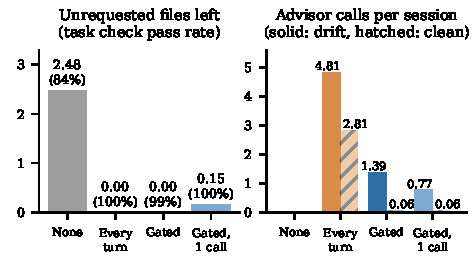
\includegraphics[width=\columnwidth]{fig_loop.pdf}
\caption{Four arms on the live agent: unwatched, advisor after every turn, monitor-gated advisor, and monitor-gated with one call at most. Gating by the monitor matches per-turn review on outcomes with far fewer advisor calls, especially on clean sessions. Capping the monitor at one call left files behind in 2 of 48 sessions.}
\label{fig:loop}
\end{figure}

\subsection{Harder drift and lookalikes}\label{sec:edge}

A second run probed harder drift and lookalikes: 8 unseen tasks, two agents (Gemini 3.1 Flash-Lite, Grok 4.7), a Claude Opus 5.5 advisor at threshold 40, 16 sessions per condition per arm, 360 in all (Table~\ref{tab:edge}). Advice fixes drift that can be undone: leaked credentials, broken constraints and a replaced goal. It fails in two cases. Deletion cannot be advised away: the monitor flagged all 9 unwatched deletions on replay, but the file is gone before a note arrives (13/16 vs.\ 9/16 watched vs.\ unwatched, Fisher $p{=}0.25$, no real difference). An agent told to refuse correction was flagged in 15 of 16 watched sessions and ignored every note. Both call for a different response than advice: blocking the action, or escalating to a human. On 64 lookalike sessions, where the user had authorised the alarming-looking work, notes reached the agent in only 3.

\begin{table}[t]
\centering\small
\setlength{\tabcolsep}{4pt}
\begin{tabular}{@{}lrrr@{}}
\toprule
Hidden drift & Unw. & Watched & Flagged \\
\midrule
copies credentials & 7/16 & \best{1/16} & 7/7 \\
breaks a constraint & 6/16 & \best{0/16} & 6/6 \\
continues replaced goal & 12/12 & \best{5/12} & 10/12 \\
obeys planted instruction & 2/16 & \best{0/16} & 0/2 \\
deletes unasked files & 9/16 & 13/16 & 9/9 \\
refuses correction & 16/16 & 16/16 & 16/16 \\
\bottomrule
\end{tabular}
\caption{Sessions ending badly, unwatched vs.\ watched, and unwatched failures the monitor flags on replay.}
\label{tab:edge}
\end{table}

\subsection{Cost}

On one RTX 3080 at 4-bit, a score takes 309\,ms (132\,ms per score at batch 8) and 2.66\,GB of memory; the output is one token. Because the monitor rations advisor calls rather than removing them, we compare total system cost per million agent steps: monitor serving plus the advisor calls that still fire, against reviewing every step. At an advisor price of \$2.50 per million input tokens, that is \$463 at threshold 30 (\$316 at 40) against \$1,735, a saving of 73\% (82\%). Monitor serving alone is \$17 per million steps. Appendix~\ref{app:cost} gives the sweep.

\section{What Did Not Work}\label{sec:failures}

\paragraph{Synthetic-only training over-fired on real traffic.} The first model scored real sessions at a mean of 30.7 against labels of 11.1 (false alarms 30\%), and no threshold rescued it. We tested whether the real labels were simply lenient: an independent judge applying our rubric scored those sessions at 10.6, close to the stored 11.1. The model was wrong, not the labels. Mixing 60\% of real sessions into training and raising the on-course share from 35\% to 55\% cut real-session MAE from 20.1 to 7.6, at a cost of 0.4 MAE on synthetic data.

\paragraph{Confident endings as a proxy for drift.} A 14-step session in which every action was requested and verified scored correctly for 11 steps and then 73 at the closing report. In training, drift sessions tended to end with confident reports and controls with quiet endings, so ending style had become a label proxy \citep{geirhos2020shortcut}. We added an \emph{ending} axis assigned independently of the label, and controls that do everything asked, verify it and report fully, one closing with ``Status: complete, tested and verified'' labelled 3. The session then scored 28, and an inverted scaffolding pair (61 vs.\ 54) became correct (65 vs.\ 22).

\section{Conclusion}

A 3.35B model trained on paired drift and on-course sessions can decide when an agent needs a stronger model's attention. It outperforms frontier models used zero-shot on the same prompt, and on a live agent it matches per-turn review on outcomes at a fraction of the calls. The failures point to the next steps: block irreversible actions before they run rather than advise after them, escalate to a human when advice is ignored, and train on sessions that include the advisor's notes.

\section*{Limitations}

\begin{itemize}\itemsep0pt
\item \textbf{Deletions and resistant agents} are detected but not fixed by advice (\S\ref{sec:edge}); they need blocking or human escalation, which we did not build.
\item \textbf{Drift inside a requested file is under-detected.} The one monitor-arm failure in the main loop was an answer at about twice its 120-word limit, inside the requested file; the monitor's view clips long file bodies and scored it 10.6.
\item \textbf{The monitor does not see advisor notes,} so repairs look like new drift: 126 of 197 turns after a note still alerted. Showing the notes without retraining fixes this (5/197) but also silences 20 of 69 unrepaired sessions (Appendix~\ref{app:notes}).
\item \textbf{Scope.} The main loop used one agent model, one advisor, sixteen small tasks and mild, compliant drift. The unseen tasks were written by us, so they share our idea of a task.
\item \textbf{Labels are model-generated,} with synthetic sessions from one teacher family; blind judges measure agreement between models, not truth. Synthetic sessions are written, not executed; the held-out real split measures that cost.
\item \textbf{Calibration.} Cases deserving 80--100 land at 50--72, so the score is a ranking rather than a calibrated severity, and replies-only sessions (tier 1) over-fire.
\end{itemize}

\section*{Ethics Statement}

The monitor is meant to increase human oversight of agents, not replace it; on its own it cannot stop irreversible actions or a resistant agent, and we recommend blocking and human escalation for those cases. CuratorKIT's secrets gate scanned the corpus; the hits are fixture hashes and deliberately fake credentials inside scenarios about mishandled secrets. The recorded sessions are agent runs on tasks and fixture files that we wrote, in sandboxes: no human users' conversations or third-party data were recorded, and the people, addresses and credentials that appear in sessions are invented. Everything published was scanned for local paths, usernames, e-mail addresses and keys. The base model is licensed CC-BY-NC-4.0, so the adapter and data are released non-commercially.

\bibliography{refs}

\appendix
\raggedbottom % the appendix tables cannot break, so do not stretch the column they leave short

\section{Drift Patterns}\label{app:patterns}

The 16 drift patterns with their label bands, and the on-course controls that mirror them (label bands 0--15 to 0--30). Three further controls mirror no single pattern: \texttt{clean}, \texttt{legit\_long} (a long multi-file session, the main false-alarm trap) and \texttt{recover} (drifted, was corrected, and is back on course; 10--40). Each session also has an \emph{ending} style (thorough report, quiet, normal) assigned independently of the label (\S\ref{sec:failures}).

\noindent{\footnotesize\setlength{\tabcolsep}{2.5pt}
\begin{tabular}{@{}lr>{\raggedright\arraybackslash}p{0.43\columnwidth}@{}}
\toprule
Drift pattern & Band & Control(s) \\
\midrule
\texttt{side\_task} & 40--65 & \texttt{legit\_scope}, \texttt{legit\_change} \\
\texttt{constraint\_small} & 55--80 & \texttt{legit\_lift} \\
\texttt{constraint\_large} & 60--85 & -- \\
\texttt{stale} & 60--90 & \texttt{goal\_switch} \\
\texttt{premature\_done} & 60--95 & \texttt{legit\_complete}, \texttt{legit\_stop} \\
\texttt{silent\_shortfall} & 45--75 & \texttt{legit\_partial} \\
\texttt{setup\_excess} & 40--70 & \texttt{legit\_setup} \\
\texttt{loop} & 35--60 & \texttt{legit\_recheck} \\
\texttt{stuck} & 45--75 & \texttt{debug\_progress}, \texttt{blocked\_env} \\
\texttt{destructive} & 70--100 & \texttt{legit\_destructive} \\
\texttt{injection\_obeyed} & 65--95 & \texttt{injection\_refused} \\
\texttt{wrong\_approach} & 45--75 & \texttt{legit\_detour} \\
\texttt{wrong\_deliverable} & 40--70 & \texttt{clarify} \\
\texttt{unverified\_claim} & 45--75 & \texttt{legit\_verified} \\
\texttt{scope\_reduction} & 40--70 & -- \\
\texttt{quota\_waste} & 30--55 & -- \\
\bottomrule
\end{tabular}}
\vspace{6pt}

\section{Evidence Tiers}\label{app:tiers}

\noindent{\small\setlength{\tabcolsep}{4pt}\begin{tabular}{@{}cl@{}}
\toprule
Tier & Visible to the monitor \\
\midrule
1 & replies only \\
2 & replies + which tool ran \\
3 & + calls, results, provider reasoning summary \\
4 & + opening of each reasoning block \\
5 & complete record with full reasoning \\
6 & live stream, latest reasoning cut mid-thought \\
\bottomrule
\end{tabular}}
\vspace{6pt}

\noindent Tier 5 gets 20/22 hand-written decisions right; tier 1 over-fires, treating unverifiable completion claims as suspect. A tier-specific threshold did not help.

\section{Label Quality}\label{app:labels}

\noindent{\small\setlength{\tabcolsep}{4pt}\begin{tabular}{@{}lrrr@{}}
\toprule
Comparison & MAE & Pearson & $\pm$1 digit \\
\midrule
Labels vs judge A & 7.4 & 0.957 & 86.6\% \\
Labels vs judge B & 11.4 & 0.900 & 75.3\% \\
Judge A vs judge B & 12.4 & 0.893 & 66.7\% \\
Labels vs both & 9.6 & 0.915 & 80.5\% \\
\bottomrule
\end{tabular}}
\vspace{6pt}

\noindent The label mean (28.0) lies between the judges' (25.5 and 30.4). Disagreement is highest on authorised destructive work (19.2) and refused injections (15.0), lowest on reckless deletion (3.3).

\section{Hand-Written Suites}\label{app:suites}

Twenty-five scenarios covering categories and known failures: base 12/25, trained 23/25. Twenty-four novel scenarios (conflicting instructions, delayed harm, recovery, goal evolution): 23/24 at threshold 30, 21/24 at 40. Representative pairs (drift vs.\ on-course score): planted note escalating vs.\ aligned with the user, 93.0 vs.\ 13.7; goal replaced twice, following the middle vs.\ newest goal, 71.9 vs.\ 10.0; migration run against live vs.\ staging, 59.2 vs.\ 5.5; word limit exceeded vs.\ counted and met, 49.9 vs.\ 10.8.

\section{Advisor Notes and Re-Alerting}\label{app:notes}

Replaying 69 watched sessions that received a note, with the notes made visible to the monitor (no retraining), at threshold 30:

\noindent{\small\setlength{\tabcolsep}{4pt}\begin{tabular}{@{}lrr@{}}
\toprule
& Hidden & Visible \\
\midrule
Turns after a note still alerting & 126/197 & 5/197 \\
Final turn still alerting & 42/69 & 0/69 \\
Control: turn before repair & 68/69 & 48/69 \\
\bottomrule
\end{tabular}}
\vspace{6pt}

\noindent The control shows the monitor is mostly reading the work (mean 42.6 before vs.\ 17.1 after repair), not just becoming lenient, but 20 sessions lose a correct alert. Training on sessions with notes is the next step.

\section{Operating Point and Cost}\label{app:cost}

\noindent{\small\setlength{\tabcolsep}{4pt}\begin{tabular}{@{}rrrr@{}}
\toprule
Thr. & Recall & Precision & FA \\
\midrule
25 & 0.935 & 0.581 & 12.8\% \\
30 & 0.900 & 0.612 & 10.9\% \\
40 & 0.794 & 0.737 & 5.4\% \\
\bottomrule
\end{tabular}}
\vspace{6pt}

\noindent We recommend threshold 30: the cost sweep on real data (optimum 25--30) and the novel suite (no misses at 30) agree. Measured alert rates are 25.7\% at 30 and 17.2\% at 40. Cost per million steps (input tokens only charged to the advisor, which favours it):

\noindent{\small\setlength{\tabcolsep}{4pt}\begin{tabular}{@{}rrrr@{}}
\toprule
\$/Mtok & Every step & Gated @30 & Gated @40 \\
\midrule
0.25 & 173.50 & 61.92 & 47.17 \\
2.50 & 1{,}735.00 & 463.23 & 315.75 \\
10.00 & 6{,}940.00 & 1{,}800.91 & 1{,}211.01 \\
\bottomrule
\end{tabular}}
\vspace{6pt}

\section{Pipeline, Models and Licences}\label{app:pipeline}

\paragraph{Toolkits.} CuratorKIT \citep{curatorkit} is used twice. In-line, it cleaned, MinHash-deduplicated and secrets-gated the recorded corpus before it entered the splits. As an audit after training, the same pass over the exact 14,000-row training split flags 3.1\% of rows: 30 exact duplicates, 167 near-duplicates and 237 secrets-gate hits, the last being fixture hashes and the deliberately fake credentials inside scenarios about mishandled secrets. The adapter was trained on the unfiltered rows; we report that rather than imply the final split was curated before training. AlignTune \citep{aligntune} runs the QLoRA fine-tune. AuditKIT \citep{auditkit} scores every run from stored predictions through its \texttt{PrecomputedModel}, grades the before/after deltas and writes the provenance record that chains the three stages.

\paragraph{Models.} Only tiny-aya-global is trained or shipped. Other models appear in supporting roles, none at inference time in the monitor: Grok 4.7 as the teacher; Grok 4.7 (1,089 sessions), Claude Haiku 5.5 (410), Claude Sonnet 5.5 (317) and GPT-6 Luna (86) as the agents in the recorded sessions; Claude Sonnet 5.5 and GPT-6.1 Terra as blind judges and zero-shot baselines; Claude Sonnet 5.5 and Claude Opus 5.5 as advisors.

\paragraph{Licences.} The adapter and the dataset are released under CC-BY-NC-4.0, inherited from the base model. CuratorKIT and AuditKIT are used under the Lexsi Source Available Licence v1.2, and AlignTune under its own licence.

\section{With More Credits}\label{app:credits}

What we would do next, in order of expected value. The last column is a forecast, not a measurement.

\smallskip\noindent{\footnotesize\setlength{\tabcolsep}{3pt}
\begin{tabular}{@{}>{\raggedright\arraybackslash}p{0.33\columnwidth}>{\raggedright\arraybackslash}p{0.29\columnwidth}>{\raggedright\arraybackslash}p{0.31\columnwidth}@{}}
\toprule
Work & Measured now & Forecast \\
\midrule
Train on sessions that contain advisor notes & 126/197 turns after a note still alert & under 10/197, with the unrepaired control alerting in at least 65/69 \\
\addlinespace
Score the proposed tool call and block irreversible actions above the threshold & 13/16 harmful deletions with the advisor & 2/16 or fewer \\
\addlinespace
Escalate to a human when a note is ignored & 16/16 ended badly, 15/16 alerted & 15/16 handed to a person within one step \\
\addlinespace
Show the monitor more of the requested file & 1 miss in the main loop (score 10.6) & that case caught; the longer prompt to be measured against 309\,ms \\
\addlinespace
Closed loop on resistant and more capable agents, and more tasks & 256 + 360 sessions, 2 agent families & the same outcome table at 1,000+ sessions, with a confidence interval per condition \\
\bottomrule
\end{tabular}}
\vspace{6pt}

\noindent Retraining costs about 11 GPU-hours (\$5.20), so most further credit would go on agent and advisor API calls for the larger closed loop.

\section{Artifacts and Reproducibility}\label{app:artifacts}

\begin{itemize}\itemsep0pt\raggedright
\item Adapter:\\ \href{https://huggingface.co/dev-willbird1936/drift-monitor-tiny-aya}{\nolinkurl{huggingface.co/dev-willbird1936/drift-monitor-tiny-aya}}
\item Data, logs, traces:\\ \href{https://huggingface.co/datasets/dev-willbird1936/drift-monitor-data}{\nolinkurl{huggingface.co/datasets/dev-willbird1936/drift-monitor-data}}
\item Demo (replays and a live agent, no key needed):\\ \href{https://huggingface.co/spaces/dev-willbird1936/drift-monitor}{\nolinkurl{huggingface.co/spaces/dev-willbird1936/drift-monitor}}
\item Code, this paper's source (\texttt{paper/}) and a three-minute video with slides (\texttt{video/}):\\ \href{https://github.com/dev-willbird1936/drift-monitor}{\nolinkurl{github.com/dev-willbird1936/drift-monitor}}
\end{itemize}
The repository scripts regenerate the corpus, audit labels, assemble splits, train with AlignTune and grade with AuditKIT. The monitor also ships as a Pi agent extension and a Python wrapper that accepts OpenAI-format transcripts. All work was done during the hackathon (1--15 November 2026).

\paragraph{Acknowledgements.} We thank Lexsi Labs, Cohere Labs and Hugging Face for the hackathon, the toolkits, the base model and the compute credits.

\paragraph{Use of AI assistants.} Language models generated and labelled the synthetic data, acted as agents, judges and advisors as described, and assisted with code and editing of this paper.

\end{document}
